
  
\documentclass[12pt,a4paper]{article}
\usepackage{amsmath,amscd,amsbsy,amssymb,latexsym,url,bm,amsthm}
\usepackage{epsfig,graphicx,subfigure}
\usepackage{enumitem,balance}
\usepackage{wrapfig}
\usepackage{mathrsfs,euscript}
\usepackage[usenames]{xcolor}
\usepackage{hyperref}
\usepackage[vlined,ruled,commentsnumbered,linesnumbered]{algorithm2e}

%note: use \setcounter{exercise}{5} to change the numbering
\theoremstyle{definition}
\newtheorem{exercise}{Exercise}
\newtheorem*{solution}{Solution}

%copied from VE281. I don't know what they are used for. Some are used to expand the margin.
\setlength{\oddsidemargin}{-0.365in}
\setlength{\evensidemargin}{-0.365in}
\setlength{\topmargin}{-0.3in}
\setlength{\headheight}{0in}
\setlength{\headsep}{0in}
\setlength{\textheight}{10.1in}
\setlength{\textwidth}{7in}
\makeatletter \renewenvironment{proof}[1][Proof] {\par\pushQED{\qed}\normalfont\topsep6\p@\@plus6\p@\relax\trivlist\item[\hskip\labelsep\bfseries#1\@addpunct{.}]\ignorespaces}{\popQED\endtrivlist\@endpefalse} \makeatother
\makeatletter
\renewenvironment{solution}[1][Solution] {\par\pushQED{\qed}\normalfont\topsep6\p@\@plus6\p@\relax\trivlist\item[\hskip\labelsep\bfseries#1\@addpunct{.}]\ignorespaces}{\popQED\endtrivlist\@endpefalse} \makeatother

\begin{document}
\title{VE401 Assignment 4}
\author{Yang, Tiancheng 517370910259\\Qiu, Yuqing 518370910026\\Chang, Siyao 517370910024}

\maketitle

\newpage

\begin{exercise}
Data Visualization
\begin{solution} \ 

    \begin{enumerate}[label=\roman*)]
        \item We use mathematica to generate this stem and leaf diagram using these data. Our code for mathematica is
        \begin{flalign*}
            \text{Needs}[\text{StatisticalPlots$\grave{ }$}]&&
        \end{flalign*}
        \begin{flalign*}
            \text{StemLeafPlot}(\text{Floor}[\text{Data},1],\text{IncludeEmptyStems}\to \text{True},\text{StemExponent}\to 1)&&
        \end{flalign*}
        \begin{center}
        \begin{tabular}{c|l}
            Stem&Leaves\\
            532&9\\
            533&\\
            534&2\\
            535&47\\
            536&6\\
            537&5678\\
            538&12345778888\\
            539&016999\\
            540&11166677889\\
            541&123666688\\
            542&0011222357899\\
            543&01111556\\
            544&00012455678\\
            545&233447899\\
            546&23569\\
            547&357\\
            548&11257\\
        \end{tabular}
        \end{center}
    
    Stem units: 10

    We comment that the diagram looks multimodal, but not symmetric.
    \item We use
    \begin{flalign*}
        \text{Histogram}[\text{Data}]&&
    \end{flalign*}
    to generate the histogram.

    \begin{figure}[htbp]
        \centering
        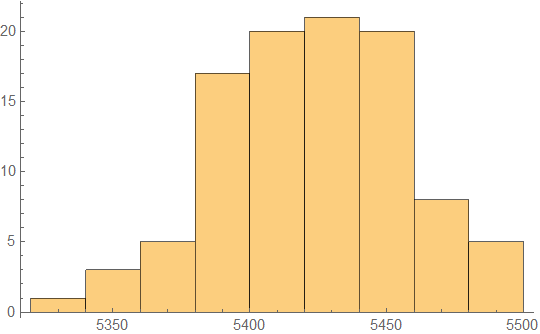
\includegraphics[width=0.5\linewidth]{E1_Histogram.png}
    \end{figure}

    The histogram looks different from the stem-and-leaf diagram. But still it looks not symmetric.
    \item We use
    \begin{flalign*}
        \text{BoxWhiskerChart[Data,\{\{"Outliers"\}\}]}&&
    \end{flalign*}
    to generate the boxplot.
    \begin{figure}[htbp]
        \centering
        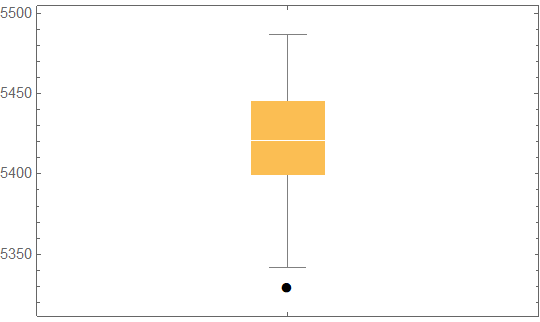
\includegraphics[width=0.5\linewidth]{E1_Boxplot.png}
    \end{figure}

    We can see that the median line is symmetric and is in the middle of the box. The whiskers don't appear to be equally long. There is only one outlier. There is strong evidence that the data follow a normal distribution, while it doesn't appear to be so in the original stem-and-leaf diagram.
\end{enumerate}    
\end{solution}
\end{exercise}
\end{document}

